\subsection{Application Tuning Parameters} \label{sec:atp}
\textbf{Intel (1 page)}
\textcolor{blue}{\begin{enumerate}
	\item Motivation
	\item How does this work? (A high level workflow, maybe?)
	\item Explain that ATPs are combined to domains and those in a domain can have constraints. 
	\begin{itemize}
		\item Manual insertion into code (ATP library). Can use runtime info to set e.g. the value space of an ATP.
		\item Pre DTA: Generation of ATP file
		\item During DTA: ATP server providing valid settings for ATPs based on the value space and the constraints.
		\item During RAT: Read by ATP library from the RRL
	\end{itemize}
\end{enumerate}}

The applications running on a cluster are aimed to solve numerical problems. Usually, the solutions can be computed with different methods. Among them there is numerical integration (Simpson, Gaussian Quadrature, Newton-Cotes, ...), function minimization (Gradient Descent, Conjugate Gradient Descent, Newton, ...) or finding the eigenvalues and eigenvectors of real matrices (power method, inverse power method, Arnoldi, ...). These methods may have different implementations, like the Fast Fourier Transform (algorithms from Cooley-Tukey, Bruun, Rader, Bluestein) implemented in the FFTW, FFTS, FFTPACK or MKL.

For a given problem, several method can provide similar numerical solution through different implementations. In HPC, the developer can chose the most efficient in term of numerical accuracy and time to solution. However, this later also depends on the computer's architecture. For example some methods can be more efficient on a vector processor than on a superscalar processor. It is up to the application's developer to chose the appropriate method and its implementation that fulfill the computer's specificity.

In the context of the energy saving, the energy consumption must also be minimized. It makes it hard for the developer to chose which method and implementation must be executed. The READEX framework let the possibility to the developer to expose the various methods and their implementation as Application Tuning Parameters. In order to pass these parameters to the tuning system, READEX provides an API to annotate the source code at locations where the tuning parameters play a role.

\begin{figure}
\centering
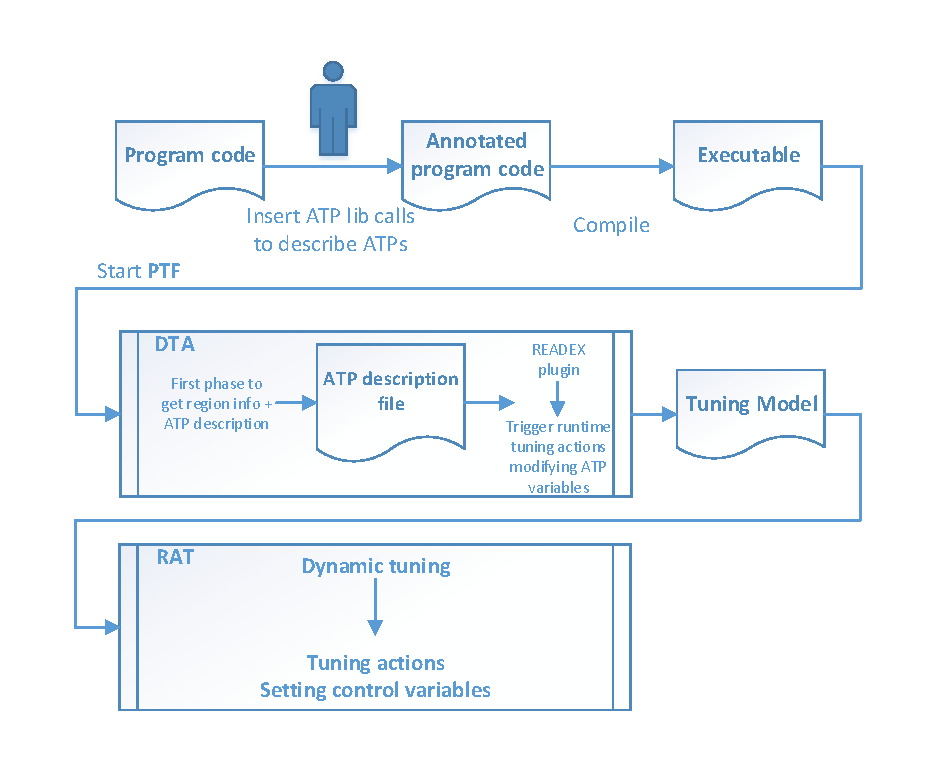
\includegraphics[width=0.8\columnwidth]{figures/overall_design.pdf} 
\caption{Workflow }
\label{fig_ATP_workflow}
\end{figure} 

The steps to handle the ATPs can be condensed in the Fig. \ref{fig_ATP_workflow}.

In details, the application developer exposes control variable and mark them as ATPs with the API functions. These functions are listed in the Listing \ref{lbl:atp_declare}.

%\vspace{0.4cm}
%\begin{minipage}{\linewidth}
%\begin{lstlisting}[caption={ATP library API functions}, label={lbl:atp_declare}]
%ATP_PARAM_DECLARE(const char *param_name, const char param_type, int default_value, const char *domain_name)
%ATP_PARAM_ADD_VALUES(const char *param_name, void *vArray, int array_size, const char *domain_name)
%---------------------------------------------------------------------------
%ATP_PARAM_GET(const char *param_name, void *atp_address, const char *domain_name)
%---------------------------------------------------------------------------
%ATP_CONSTRAINT_DECLARE(const char *constraint_name, const char *constraint_expr, const char *domain_name)
%ATP_EXPLORATION_DECLARE(const char *explorations_list, const char *domain_name)
%\end{lstlisting}
%\end{minipage}

At the moment, the ATP library handles only integers. If the required ATP has another variable type, the user must map the space of non-integer type values to integers.

The function \texttt{ATP\_PARAM\_DECLARE} declares the parameter's name, type, default value and domain. The function \texttt{ATP\_PARAM\_ADD\_VALUES} allows to add possible values the parameter can take, in a range specified by minimal, maximal and increment values ; or by enumerating explicitly the possible values.

Several ATPs can be defined in the same code. They may be independent or not. In the latter case, there is a notion of constraints between the parameters. To indicate to READEX that parameters have constraints between them, these parameters are put in the same \texttt{domain\_name}.

Listing~\ref{lbl:atp_example} shows an example of manual annotation of some generic functions. The example shows how the parameter is transfered from the tuning system through the function \texttt{ATP\_PARAM\_GET} and how the constraints are 
defined through the function \texttt{ATP\_CONSTRAINT\_DECLARE}.
	\definecolor{mygray}{rgb}{0.46,0.46,0.46}
	\lstset{language=[90]Fortran,
		%	basicstyle=\ttfamily,
		frame=lines,
		xleftmargin=\parindent,
		aboveskip=2mm,
		belowskip=2mm,
		showstringspaces=false,
		columns=flexible,
		breaklines=true,
		breakatwhitespace=true,
		keywordstyle=\color{blue},
		commentstyle=\color{mygray},
		numbers=left,
		numberstyle=\tiny\color{mygray},
		numbersep=1em,
		escapeinside={(@*}{*@)},
	}
\todo{somehow, the listing has no number. why?}
\begin{multicols}{2}[\captionof{lstlisting}{ATP constraint and exploration declaration with the ATP library.}] \label{lbl:atp_example}
\begin{lstlisting}[language=C,xleftmargin=3em,frame=none,title=\phantom{xxx}]
void foo(){
  int atp_cv;
  ...
  ATP_PARAM_DECLARE("solver", RANGE, 1, "DOM1");
  int32_t solver_values[3] = {1,5,1};
  ATP_ADD_VALUES("solver", solver_values, 3, "DOM1");
  ATP_PARAM_GET("solver", &atp_cv, "DOM1");
	
  switch (atp_cv){
  case 1:
    // choose solver 1
    break;
  case 2:
    // choose solver 2
    break;
    ...
  }
  int32_t hint_array = {GENETIC, RANDOM};
  ATP_EXPLORATION_DECLARE(hint_array, "DOM1");
}
	
void bar(){
  int atp_ms;
  ...
  ATP_PARAM_DECLARE("mesh", RANGE, 40, "DOM1");
  int32_t mesh_values[3] = {0,80,10};
  ATP_ADD_VALUES("mesh", mesh_values, 3, "DOM1");
  ATP_PARAM_GET("mesh", &atp_ms, "DOM1");
  ATP_CONSTRAINT_DECLARE("const1", "(solver = 1 && 0 <= mesh <= 40) || (solver = 2 && 40 <= mesh <= 80) || (solver > 2 && mesh = 120)", "DOM1");
  if((atp_ms > 1) && (atp_ms <= 40)){
    // choose mesh size 1
  }
  if((atp_ms > 40) && (atp_ms <= 80)){
    // choose mesh size 2
  }
  if(atp_ms == 120){
    // choose mesh size 3
  }
}
\end{lstlisting}
\end{multicols}

Once the source code is annotated and the compiled code is executed, the ATP library generates a description file in which the ATPs are written. This file contains the details about the declared application parameters.

During DTA, PTF launches the ATP server that reads the ATP description file. The ATP server's task is to respond to PTF requests, such as providing the list of ATPs or a list of valid values of ATPs. The \textit{readex\_intraphase} tuning plugin uses the list of valid values to generate a search space of the tuning parameters (not only the ATPs) and explore it. The resulting tuning model also consists of the best combination of the ATPs.

The RRL uses the ATP library during the production run to apply the best configuration. 


%	Explain that ATPs are combined to domains and those in a domain can have constraints. 
%		Manual insertion into code (ATP library). Can use runtime info to set e.g. the value space of an ATP.
%		Pre DTA: Generation of ATP file
%		During DTA: ATP server providing valid settings for ATPs based on the value space and the constraints.
%		During RAT: Read by ATP library from the RRL


